\section{The Product}
DeskSimV2 as a product is a functional simulator and a building tool for the simulator. The following section will provide a representation of both the simulator and the building tool.

The log in screen displays a basic user interface where the user will use their credentials to log in and gain access to the simulator. \\
\bigskip
\begin{figure}[H]
    \centering
    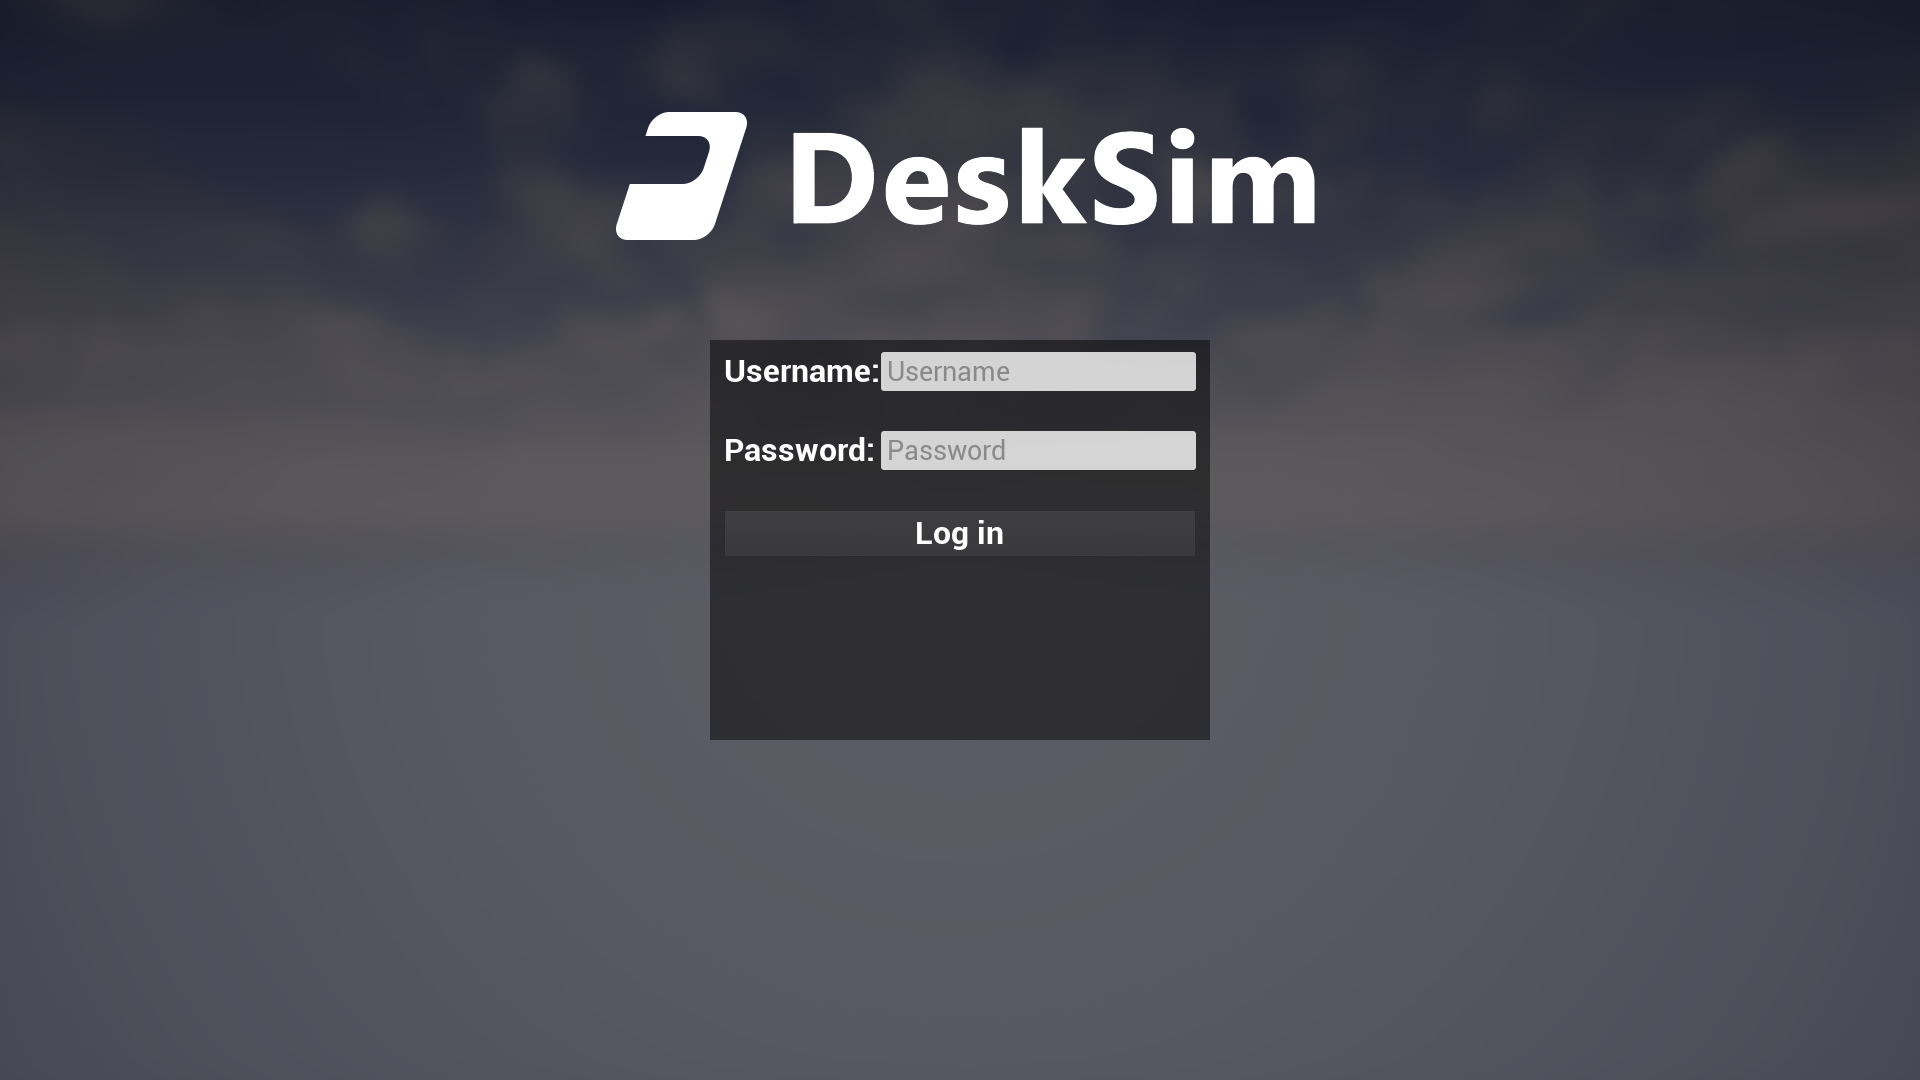
\includegraphics[width=8cm]{figures/LogIn.PNG}
    \caption{DeskSimV2: Log in Screen}
    \label{Log_in_menu_img}
\end{figure} 
\bigskip \bigskip
The main menu allows the user to select the level/scenario they want to run.
If the user has admin or teacher privileges they have the option to start a level/scenario in editing mode as well. This is shown as the "Editor" button in figure \ref{Main_Menu_img}. \\
\bigskip
\begin{figure}[H]
    \centering
    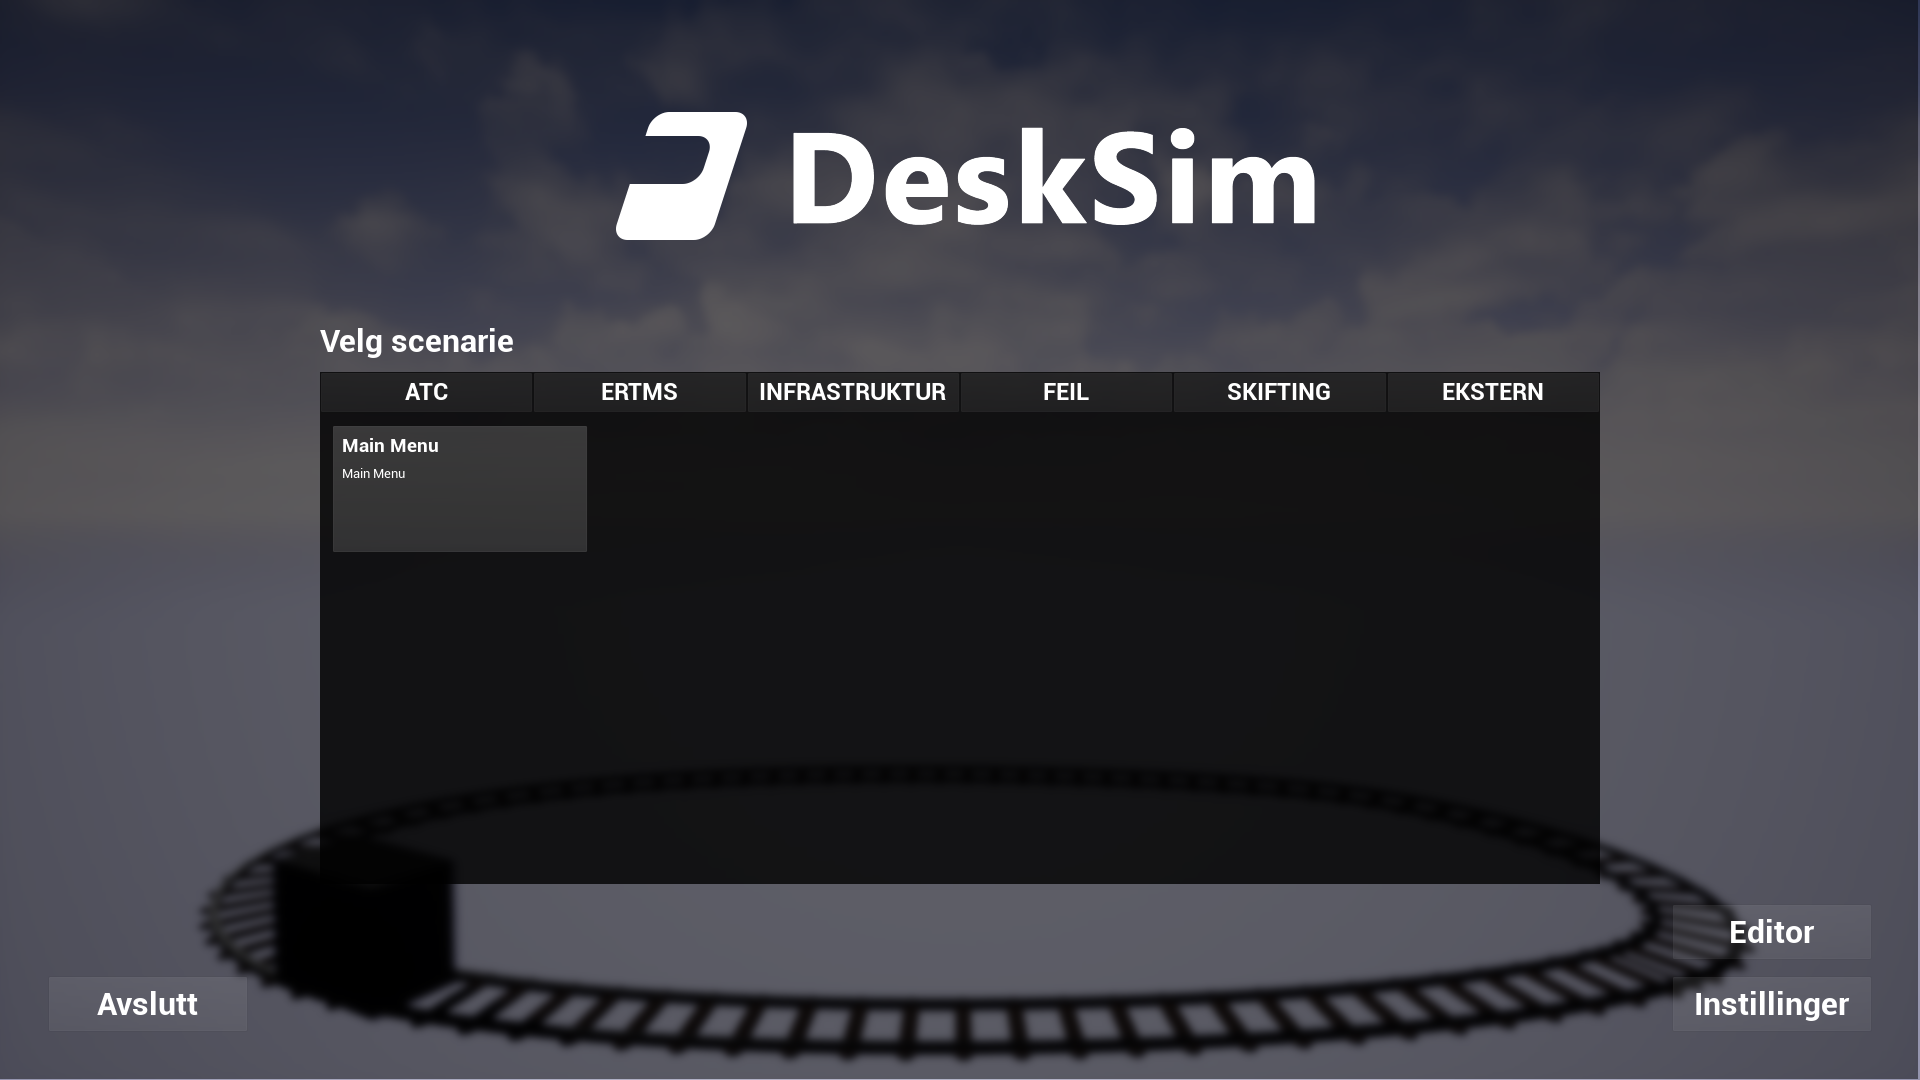
\includegraphics[width=8cm]{figures/Main Menu.PNG}
    \vspace{12pt}
    \caption{DeskSimV2: Main Menu}
    \label{Main_Menu_img}
\end{figure} 
\bigskip \bigskip
The settings menu allows the user to change the resolution and the window mode for the application
\bigskip
\begin{figure}[H]
    \centering
    \vspace{12pt}
    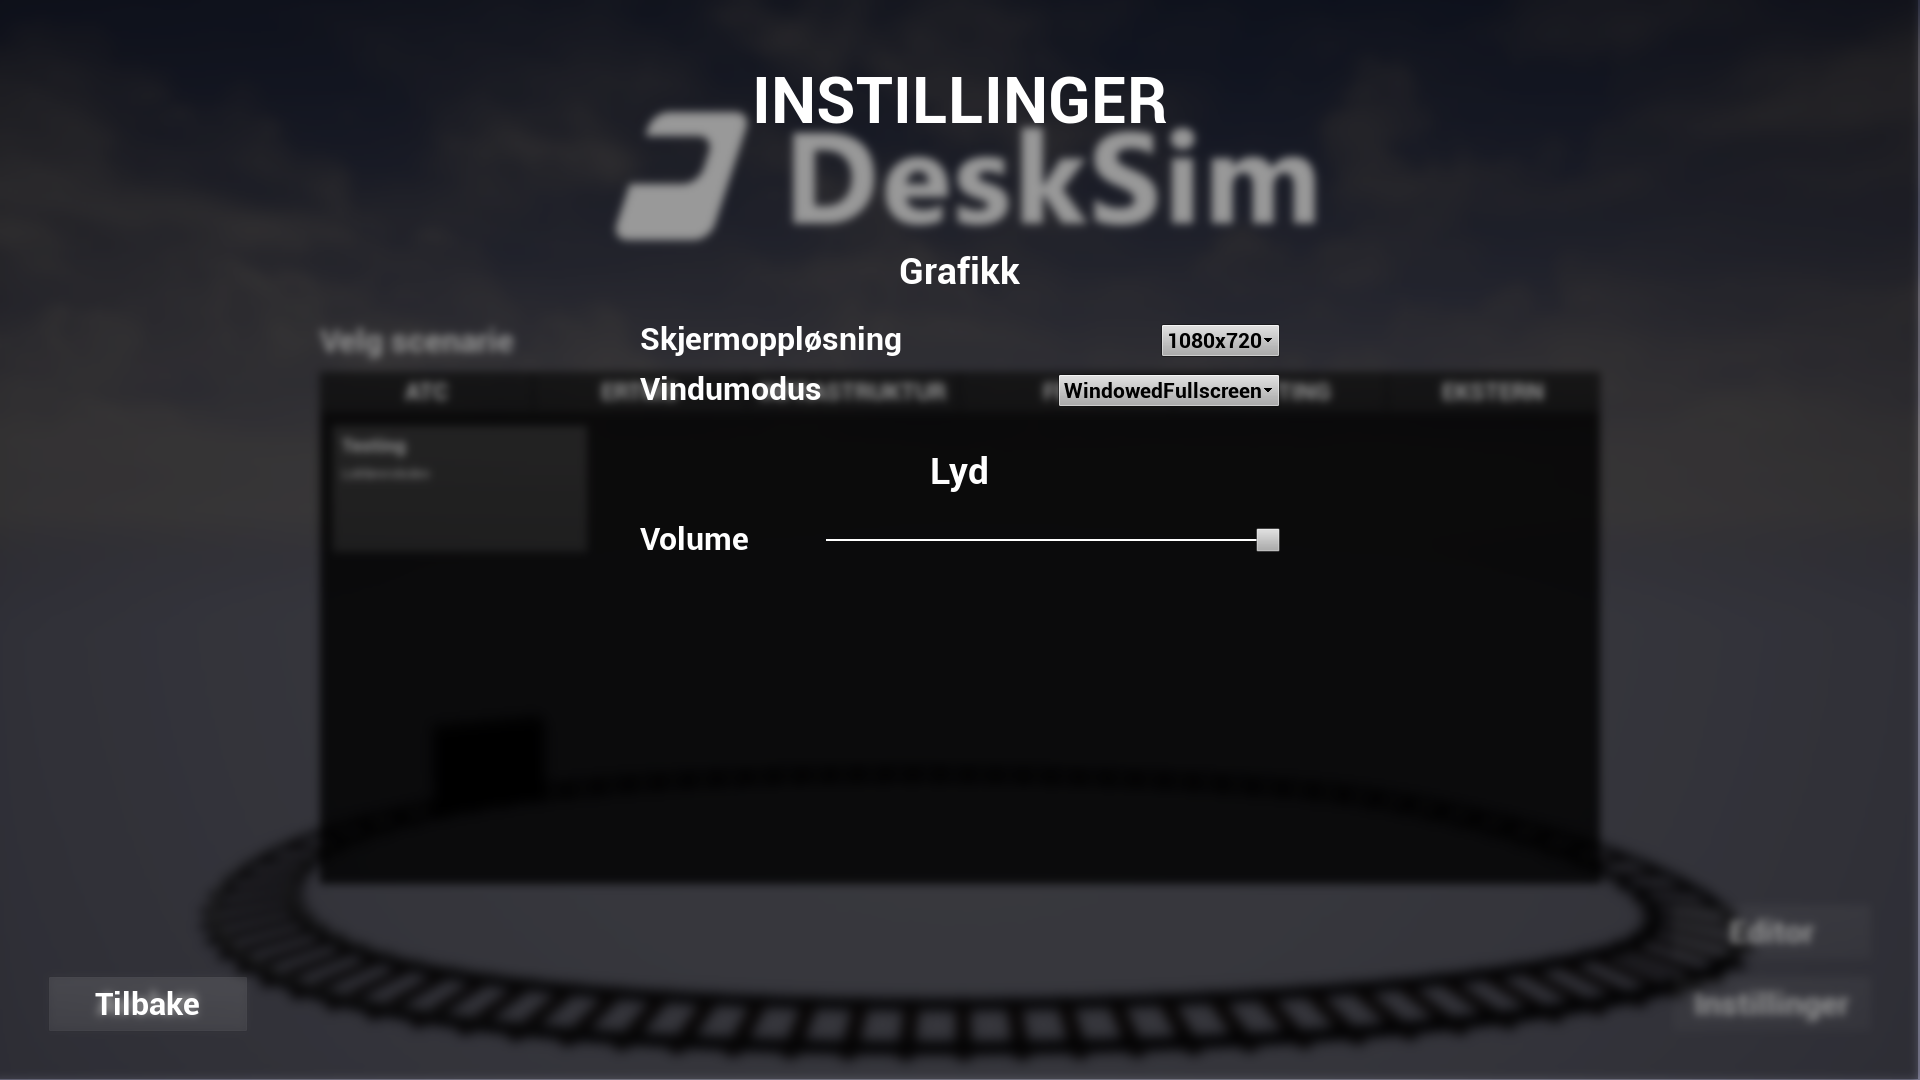
\includegraphics[width=8cm]{figures/Settings.PNG}
    %\vspace{-12pt}
    \caption{DeskSimV2: Settings Menu}
    \label{Settings_img}
\end{figure} 

The in-game experience consist of a view that corresponds to the view a train driver has from inside the front wagon of a train.
\bigskip
\begin{figure}[H]
    \centering
    \vspace{12pt}
    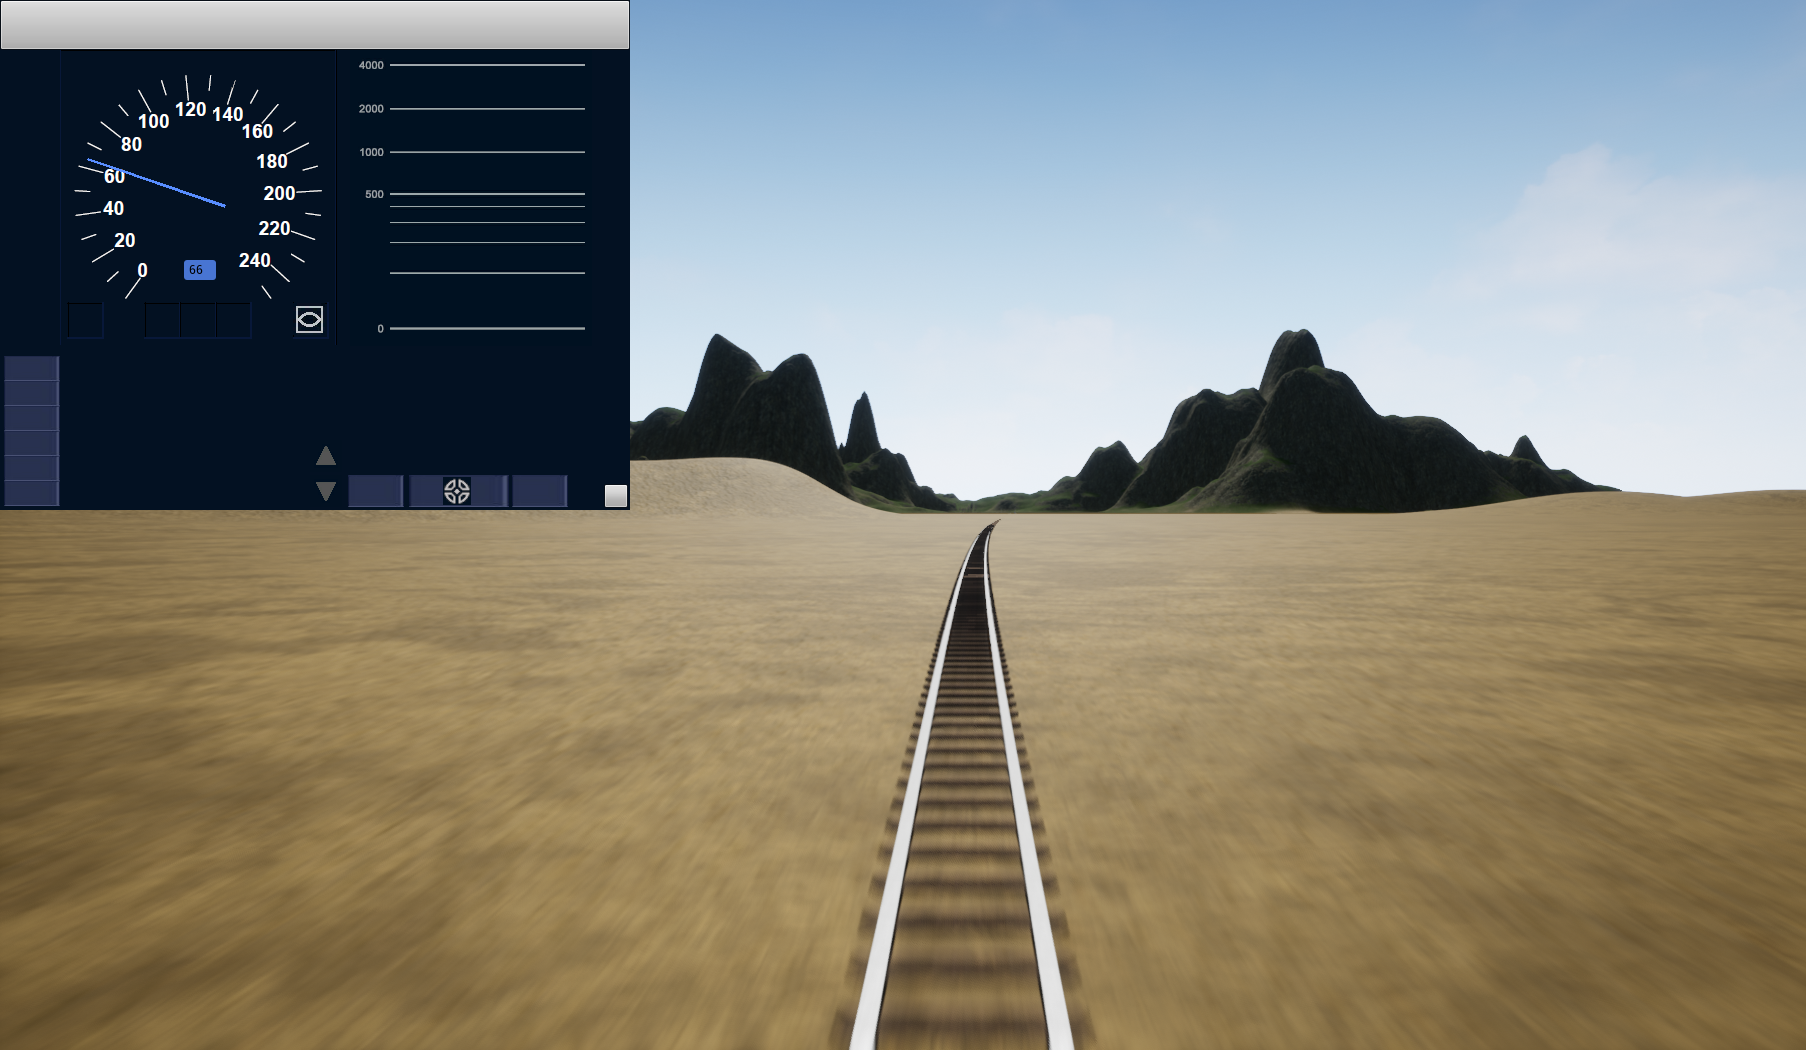
\includegraphics[width=8cm]{figures/Tog Drive.PNG}
    %\vspace{-12pt}
    \caption{DeskSimV2: Train Driver View}
    \label{Train_Driver_View_img}
\end{figure}
\bigskip \bigskip

The user will encounter different signals when running a level/scenario. The signal status and logic are predecided controlled through invisible triggerboxes and logic. 


\begin{figure}[H]
    \centering
    \vspace{12pt}
    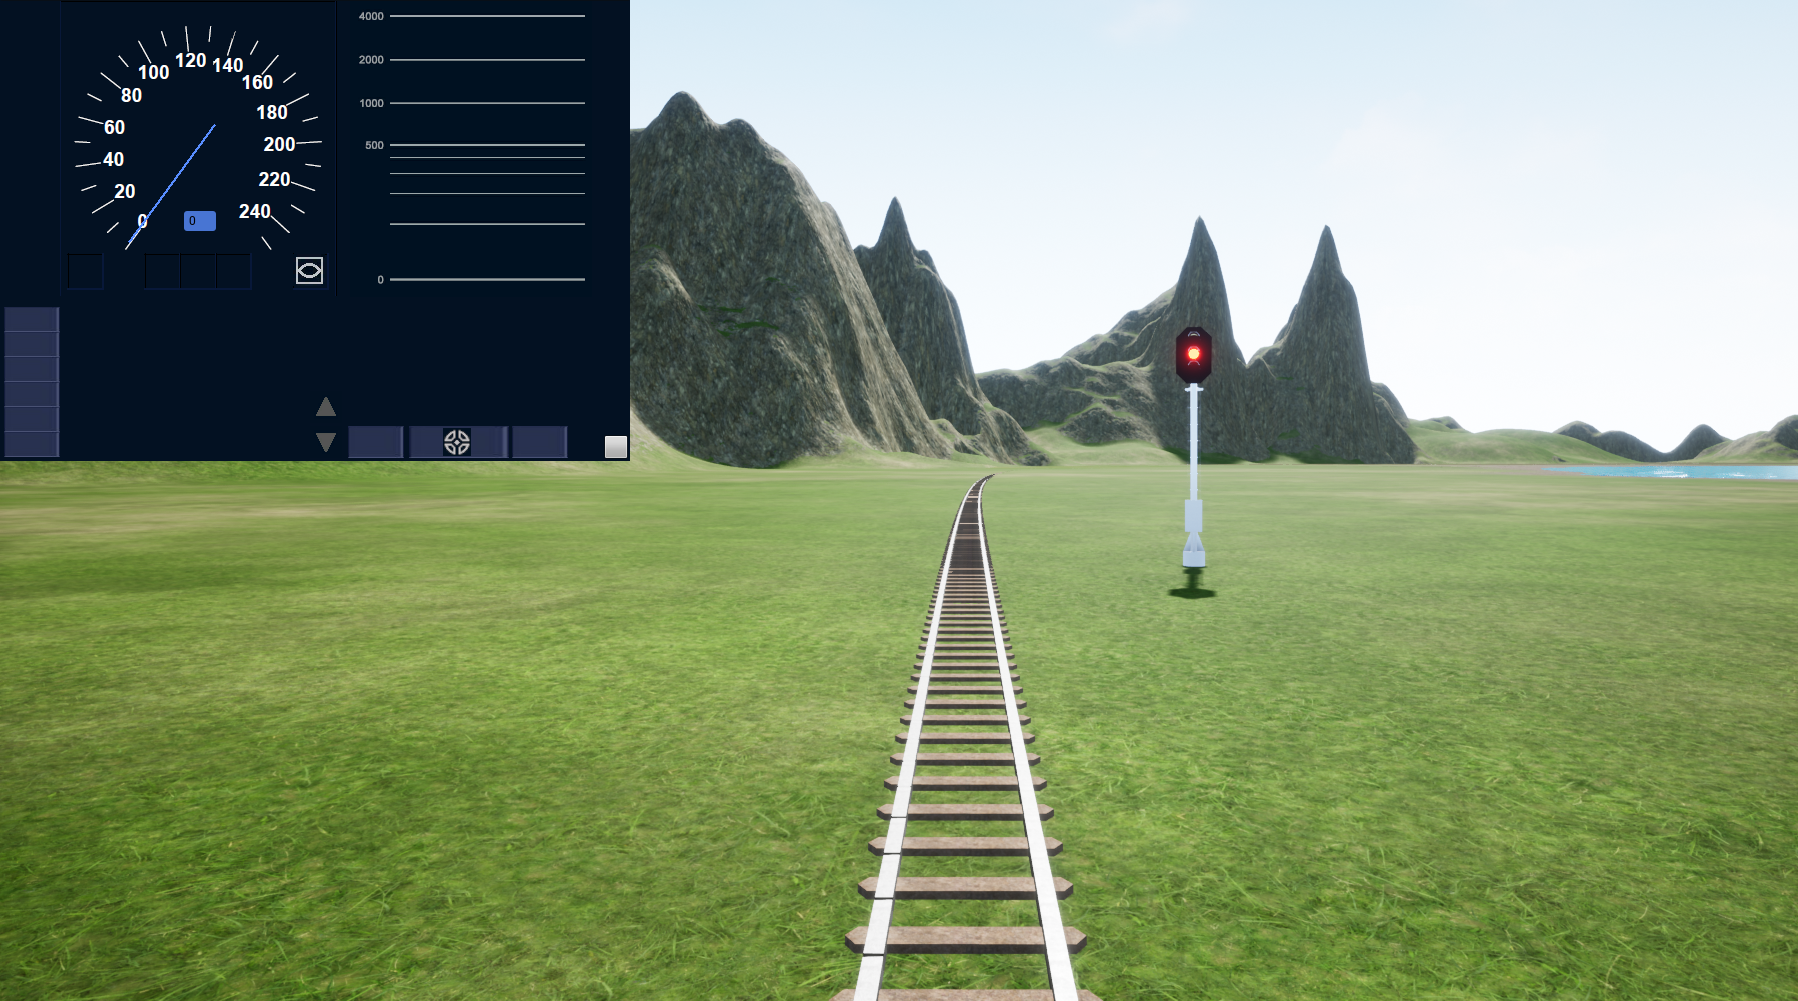
\includegraphics[width=6cm]{figures/Signal stop.PNG}
    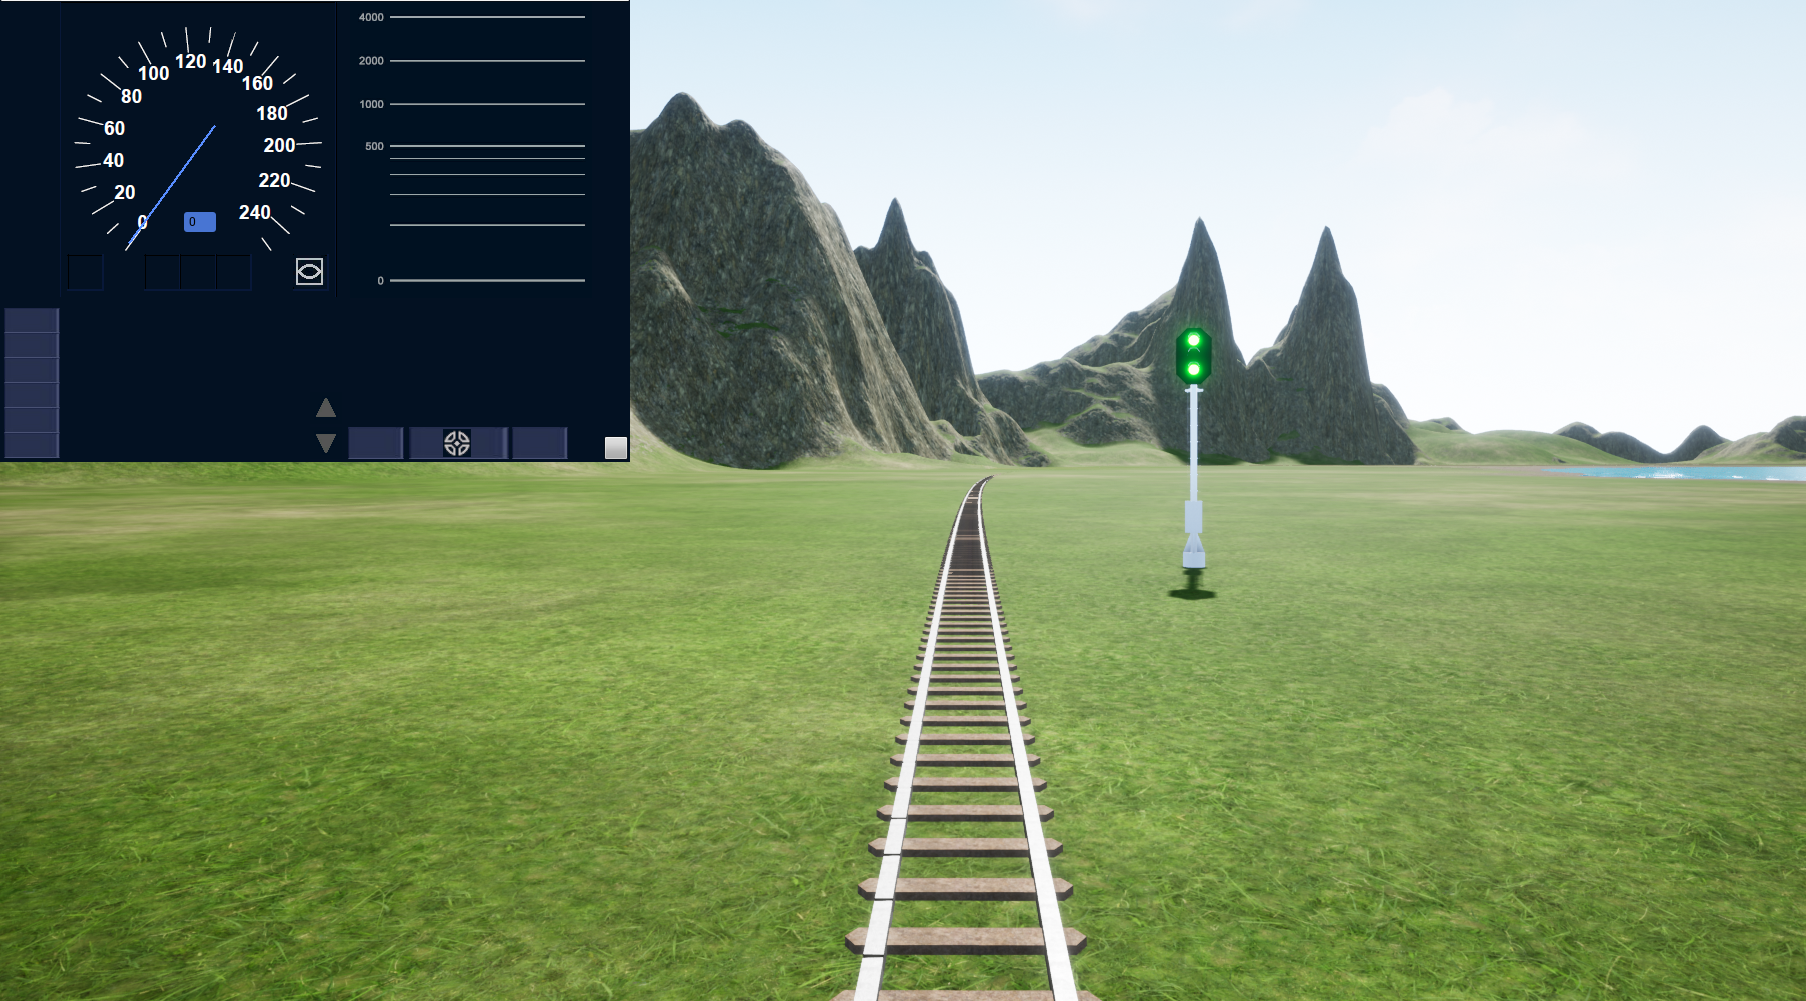
\includegraphics[width=6cm]{figures/SignalStartcorr.png}
    %\vspace{-12pt}
    \caption{DeskSimV2: Stop Signal}
    \label{Stop_Signal_img}
\end{figure} 
\bigskip \bigskip

The simulator provides an option to the user to see the world in a drone mode.
\bigskip
\begin{figure}[H]
    \centering
    \vspace{12pt}
    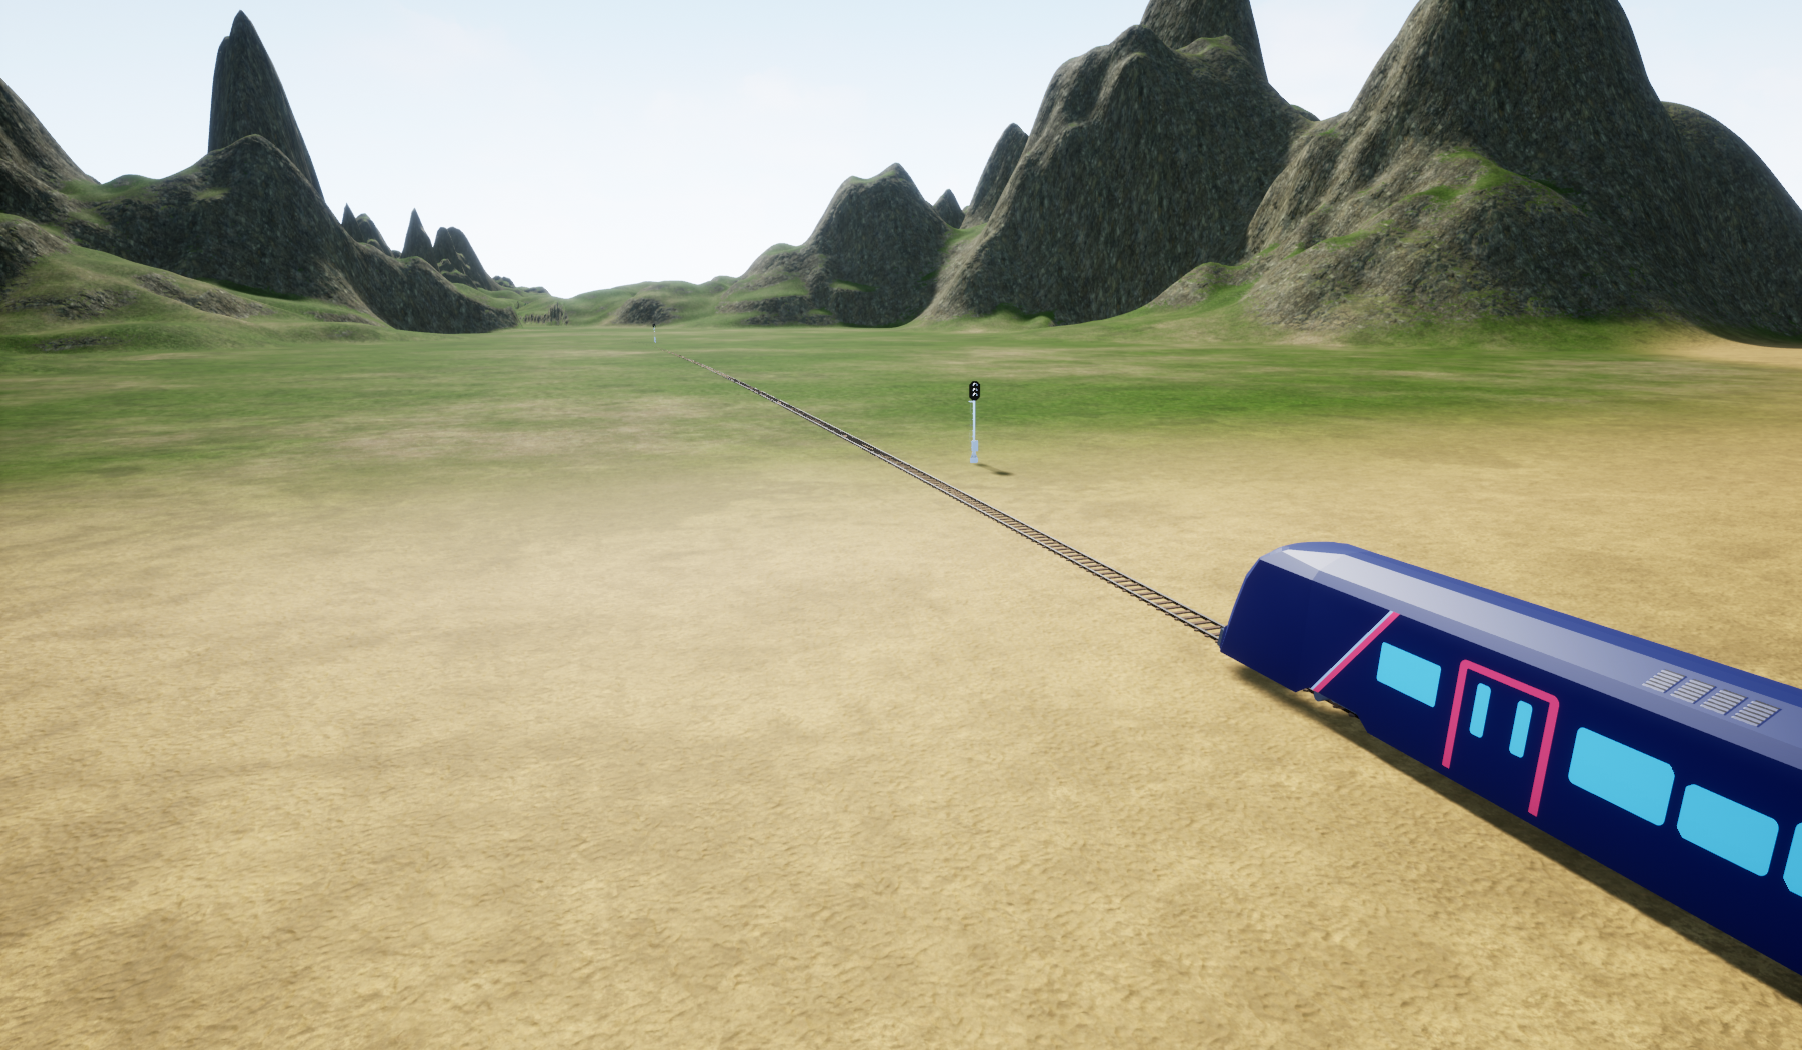
\includegraphics[width=6cm]{figures/DroneMode.PNG}
    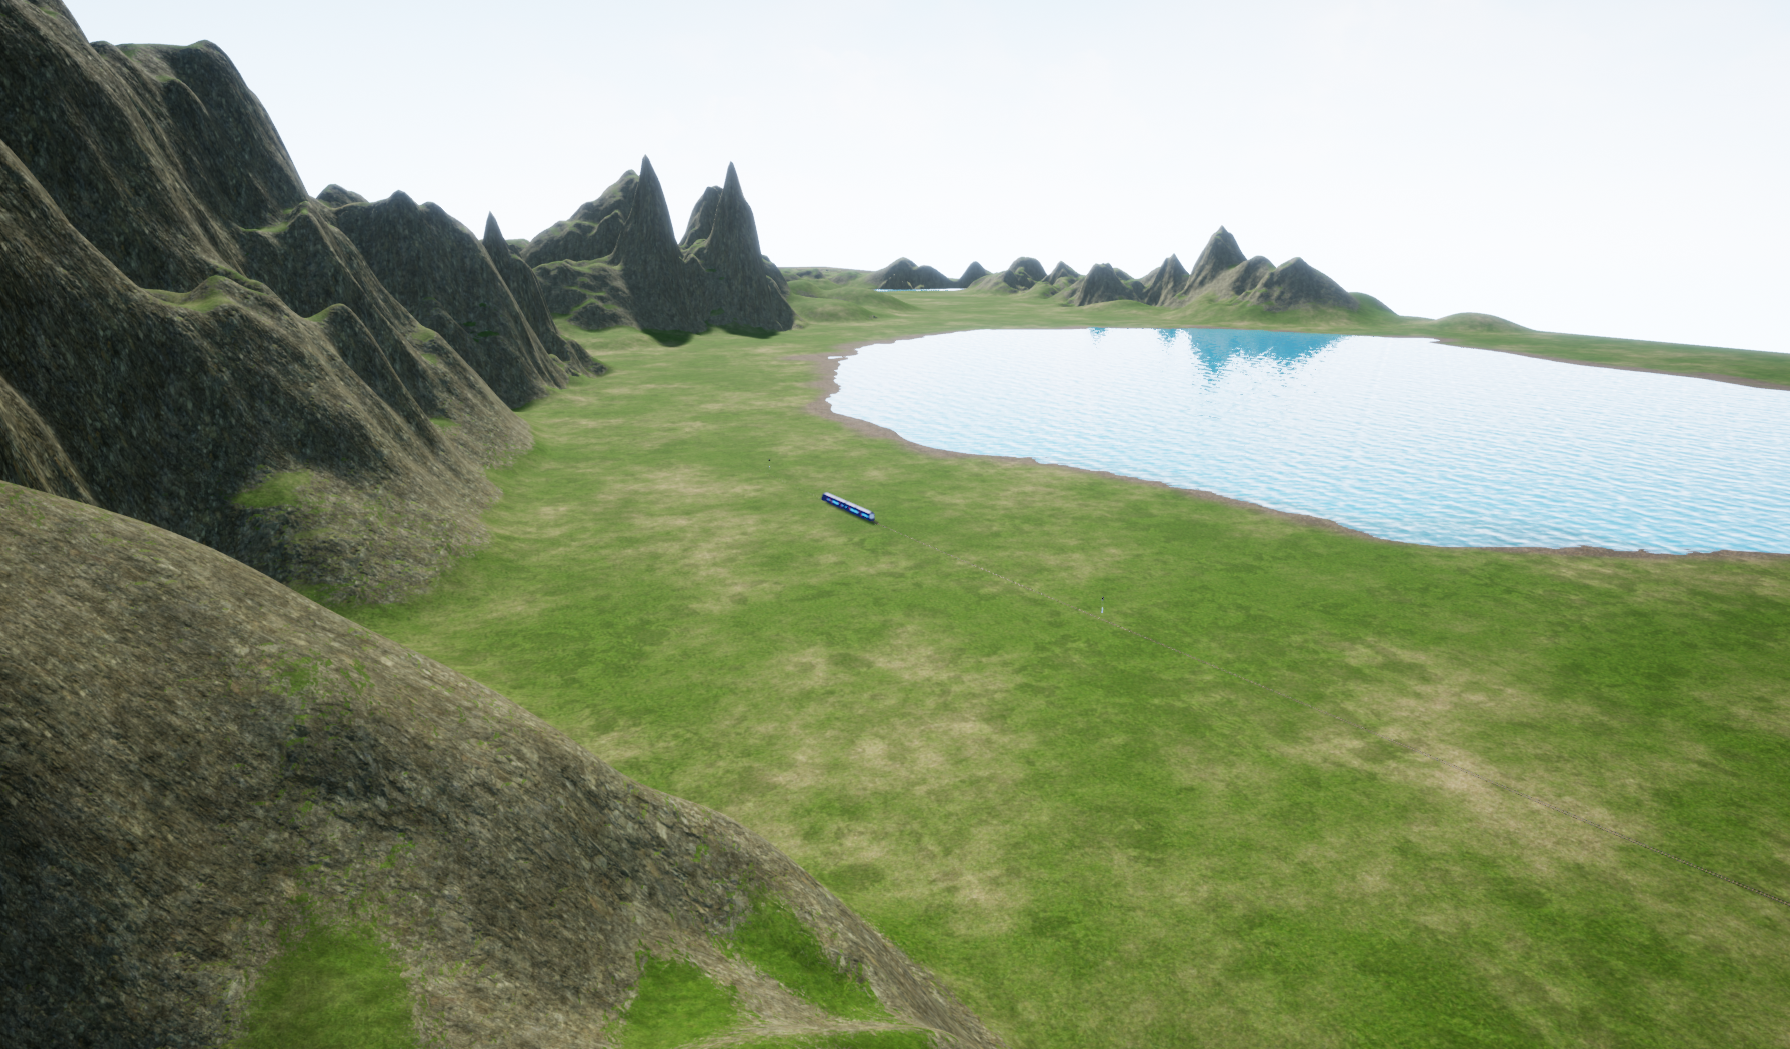
\includegraphics[width=6cm]{figures/DroneMode2.PNG}
    %\vspace{-12pt}
    \caption{DeskSimV2: Drone View}
    \label{Drone_Mode_img}
\end{figure} 
\bigskip \bigskip

The editor mode consists of a topbar where you can save your changes, change the tool mode used for objects and a trash symbol for removing objects. The other part of the User interface is the content browser where the user can drag and drop items into the level.
\bigskip
\begin{figure}[H]
    \centering
    \vspace{12pt}
    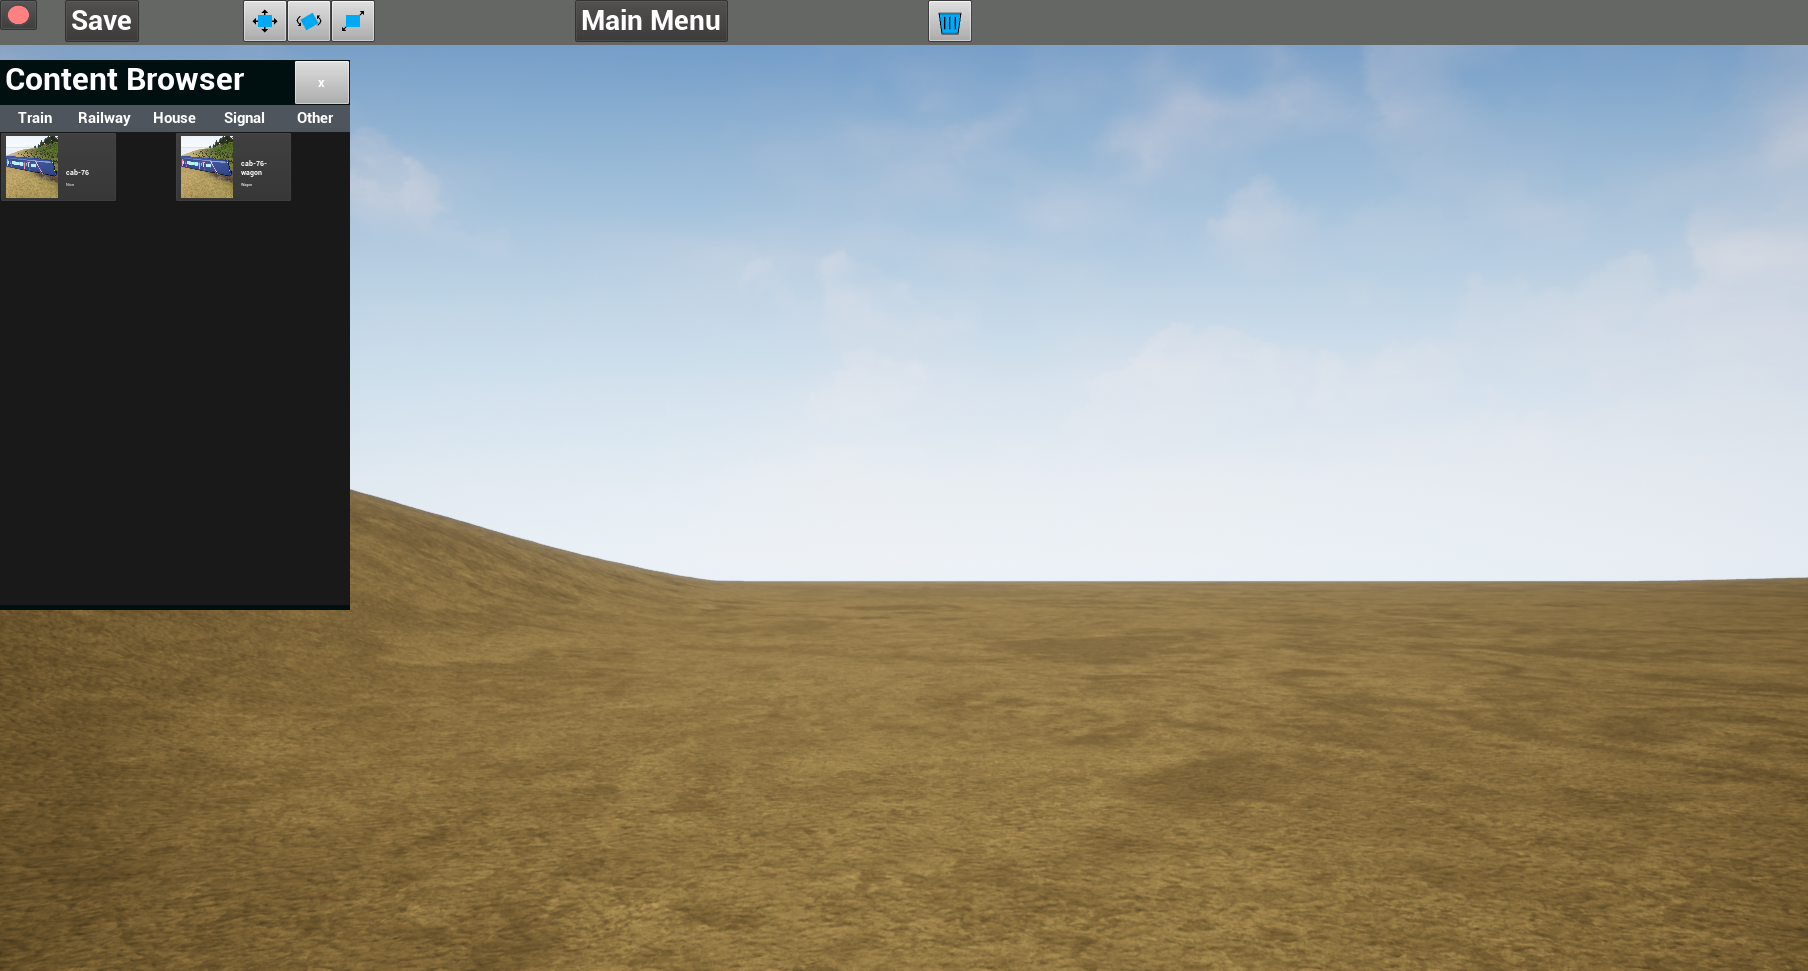
\includegraphics[width=6cm]{figures/Editor_Mode.PNG}
    %\vspace{-12pt}
    \caption{DeskSimV2: Editor Mode}
    \label{Editor_Mode_img}
\end{figure} 

\subsection{Core Functionalities}

\subsection{Menus and ui}